\documentclass{article} 
% Idioma y codificación
\usepackage[spanish, es-tabla]{babel}       %es-tabla para que se titule "Tabla"
\usepackage[utf8]{inputenc}

% Márgenes
\usepackage[a4paper,top=3cm,bottom=2.5cm,left=3cm,right=3cm]{geometry}

% Comentarios de bloque
\usepackage{verbatim}

% Paquetes de links
\usepackage[hidelinks]{hyperref}    % Permite enlaces
\usepackage{url}                    % redirecciona a la web

% Más opciones para enumeraciones
\usepackage{enumitem}

% Personalizar la portada
\usepackage{titling}


% Paquetes de tablas
\usepackage{multirow}


%------------------------------------------------------------------------

%Paquetes de figuras
\usepackage{caption}
\usepackage{subcaption} % Figuras al lado de otras
\usepackage{float}      % Poner figuras en el sitio indicado H.


% Paquetes de imágenes
\usepackage{graphicx}       % Paquete para añadir imágenes
\usepackage{transparent}    % Para manejar la opacidad de las figuras

% Paquete para usar colores
\usepackage[dvipsnames]{xcolor}
\usepackage{pagecolor}      % Para cambiar el color de la página

% Habilita tamaños de fuente mayores
\usepackage{fix-cm}


%------------------------------------------------------------------------

% Paquetes de matemáticas
\usepackage{mathtools, amsfonts, amssymb, mathrsfs}
\usepackage[makeroom]{cancel}     % Simplificar tachando
\usepackage{polynom}    % Divisiones y Ruffini
\usepackage{units} % Para poner fracciones diagonales con \nicefrac

\usepackage{pgfplots}   %Representar funciones
\pgfplotsset{compat=1.18}  % Versión 1.18

\usepackage{tikz-cd}    % Para usar diagramas de composiciones
\usetikzlibrary{calc}   % Para usar cálculo de coordenadas en tikz

%Definición de teoremas, etc.
\usepackage{amsthm}
%\swapnumbers   % Intercambia la posición del texto y de la numeración

\theoremstyle{plain}

\makeatletter
\@ifclassloaded{article}{
  \newtheorem{teo}{Teorema}[section]
}{
  \newtheorem{teo}{Teorema}[chapter]  % Se resetea en cada chapter
}
\makeatother

\newtheorem{coro}{Corolario}[teo]           % Se resetea en cada teorema
\newtheorem{prop}[teo]{Proposición}         % Usa el mismo contador que teorema
\newtheorem{lema}[teo]{Lema}                % Usa el mismo contador que teorema

\theoremstyle{remark}
\newtheorem*{observacion}{Observación}

\theoremstyle{definition}

\makeatletter
\@ifclassloaded{article}{
  \newtheorem{definicion}{Definición} [section]     % Se resetea en cada chapter
}{
  \newtheorem{definicion}{Definición} [chapter]     % Se resetea en cada chapter
}
\makeatother

\newtheorem*{notacion}{Notación}
\newtheorem*{ejemplo}{Ejemplo}
\newtheorem*{ejercicio*}{Ejercicio}             % No numerado
\newtheorem{ejercicio}{Ejercicio} [section]     % Se resetea en cada section


% Modificar el formato de la numeración del teorema "ejercicio"
\renewcommand{\theejercicio}{%
  \ifnum\value{section}=0 % Si no se ha iniciado ninguna sección
    \arabic{ejercicio}% Solo mostrar el número de ejercicio
  \else
    \thesection.\arabic{ejercicio}% Mostrar número de sección y número de ejercicio
  \fi
}


% \renewcommand\qedsymbol{$\blacksquare$}         % Cambiar símbolo QED
%------------------------------------------------------------------------

% Paquetes para encabezados
\usepackage{fancyhdr}
\pagestyle{fancy}
\fancyhf{}

\newcommand{\helv}{ % Modificación tamaño de letra
\fontfamily{}\fontsize{12}{12}\selectfont}
\setlength{\headheight}{15pt} % Amplía el tamaño del índice


%\usepackage{lastpage}   % Referenciar última pag   \pageref{LastPage}
\fancyfoot[C]{\thepage}

%------------------------------------------------------------------------

% Conseguir que no ponga "Capítulo 1". Sino solo "1."
\makeatletter
\@ifclassloaded{book}{
  \renewcommand{\chaptermark}[1]{\markboth{\thechapter.\ #1}{}} % En el encabezado
    
  \renewcommand{\@makechapterhead}[1]{%
  \vspace*{50\p@}%
  {\parindent \z@ \raggedright \normalfont
    \ifnum \c@secnumdepth >\m@ne
      \huge\bfseries \thechapter.\hspace{1em}\ignorespaces
    \fi
    \interlinepenalty\@M
    \Huge \bfseries #1\par\nobreak
    \vskip 40\p@
  }}
}
\makeatother

%------------------------------------------------------------------------
% Paquetes de cógido
\usepackage{minted}
\renewcommand\listingscaption{Código fuente}

\usepackage{fancyvrb}
% Personaliza el tamaño de los números de línea
\renewcommand{\theFancyVerbLine}{\small\arabic{FancyVerbLine}}

% Estilo para C++
\newminted{cpp}{
    frame=lines,
    framesep=2mm,
    baselinestretch=1.2,
    linenos,
    escapeinside=||
}



\usepackage{listings} % Para incluir código desde un archivo

\renewcommand\lstlistingname{Código Fuente}
\renewcommand\lstlistlistingname{Índice de Códigos Fuente}

% Definir colores
\definecolor{vscodepurple}{rgb}{0.5,0,0.5}
\definecolor{vscodeblue}{rgb}{0,0,0.8}
\definecolor{vscodegreen}{rgb}{0,0.5,0}
\definecolor{vscodegray}{rgb}{0.5,0.5,0.5}
\definecolor{vscodebackground}{rgb}{0.97,0.97,0.97}
\definecolor{vscodelightgray}{rgb}{0.9,0.9,0.9}

% Configuración para el estilo de C similar a VSCode
\lstdefinestyle{vscode_C}{
  backgroundcolor=\color{vscodebackground},
  commentstyle=\color{vscodegreen},
  keywordstyle=\color{vscodeblue},
  numberstyle=\tiny\color{vscodegray},
  stringstyle=\color{vscodepurple},
  basicstyle=\scriptsize\ttfamily,
  breakatwhitespace=false,
  breaklines=true,
  captionpos=b,
  keepspaces=true,
  numbers=left,
  numbersep=5pt,
  showspaces=false,
  showstringspaces=false,
  showtabs=false,
  tabsize=2,
  frame=tb,
  framerule=0pt,
  aboveskip=10pt,
  belowskip=10pt,
  xleftmargin=10pt,
  xrightmargin=10pt,
  framexleftmargin=10pt,
  framexrightmargin=10pt,
  framesep=0pt,
  rulecolor=\color{vscodelightgray},
  backgroundcolor=\color{vscodebackground},
}

%------------------------------------------------------------------------

% Comandos definidos
\newcommand{\bb}[1]{\mathbb{#1}}
\newcommand{\cc}[1]{\mathcal{#1}}

% I prefer the slanted \leq
\let\oldleq\leq % save them in case they're every wanted
\let\oldgeq\geq
\renewcommand{\leq}{\leqslant}
\renewcommand{\geq}{\geqslant}

% Si y solo si
\newcommand{\sii}{\iff}

% Letras griegas
\newcommand{\eps}{\epsilon}
\newcommand{\veps}{\varepsilon}
\newcommand{\lm}{\lambda}

\newcommand{\ol}{\overline}
\newcommand{\ul}{\underline}
\newcommand{\wt}{\widetilde}
\newcommand{\wh}{\widehat}

\let\oldvec\vec
\renewcommand{\vec}{\overrightarrow}

% Derivadas parciales
\newcommand{\del}[2]{\frac{\partial #1}{\partial #2}}
\newcommand{\Del}[3]{\frac{\partial^{#1} #2}{\partial^{#1} #3}}
\newcommand{\deld}[2]{\dfrac{\partial #1}{\partial #2}}
\newcommand{\Deld}[3]{\dfrac{\partial^{#1} #2}{\partial^{#1} #3}}


\newcommand{\AstIg}{\stackrel{(\ast)}{=}}
\newcommand{\Hop}{\stackrel{L'H\hat{o}pital}{=}}

\newcommand{\red}[1]{{\color{red}#1}} % Para integrales, destacar los cambios.

% Método de integración
\newcommand{\MetInt}[2]{
    \left[\begin{array}{c}
        #1 \\ #2
    \end{array}\right]
}

% Declarar aplicaciones
% 1. Nombre aplicación
% 2. Dominio
% 3. Codominio
% 4. Variable
% 5. Imagen de la variable
\newcommand{\Func}[5]{
    \begin{equation*}
        \begin{array}{rrll}
            #1:& #2 & \longrightarrow & #3\\
               & #4 & \longmapsto & #5
        \end{array}
    \end{equation*}
}

%------------------------------------------------------------------------

% Define a custom command for email addresses
\newcommand{\email}[1]{\href{mailto:#1}{{{\color{blue}#1}}}}


\usepackage{schemata}
\usepackage{ragged2e}
\usepackage{booktabs}

\newcommand{\myparagraph}[1]{\paragraph{#1}\mbox{}\\}


\begin{document}

    % 1. Foto de fondo
    % 2. Título
    % 3. Encabezado Izquierdo
    % 4. Color de fondo
    % 5. Coord x del titulo
    % 6. Coord y del titulo
    % 7. Fecha
    % 8. Autor

    
    % 1. Foto de fondo
% 2. Título
% 3. Encabezado Izquierdo
% 4. Color de fondo
% 5. Coord x del titulo
% 6. Coord y del titulo
% 7. Fecha

\newcommand{\portada}[7]{

    \portadaBase{#1}{#2}{#3}{#4}{#5}{#6}{#7}
    \portadaBook{#1}{#2}{#3}{#4}{#5}{#6}{#7}
}

\newcommand{\portadaExamen}[7]{

    \portadaBase{#1}{#2}{#3}{#4}{#5}{#6}{#7}
    \portadaArticle{#1}{#2}{#3}{#4}{#5}{#6}{#7}
}




\newcommand{\portadaBase}[7]{

    % Tiene la portada principal y la licencia Creative Commons
    
    % 1. Foto de fondo
    % 2. Título
    % 3. Encabezado Izquierdo
    % 4. Color de fondo
    % 5. Coord x del titulo
    % 6. Coord y del titulo
    % 7. Fecha
    
    
    \thispagestyle{empty}               % Sin encabezado ni pie de página
    \newgeometry{margin=0cm}        % Márgenes nulos para la primera página
    
    
    % Encabezado
    \fancyhead[L]{\helv #3}
    \fancyhead[R]{\helv \nouppercase{\leftmark}}
    
    
    \pagecolor{#4}        % Color de fondo para la portada
    
    \begin{figure}[p]
        \centering
        \transparent{0.3}           % Opacidad del 30% para la imagen
        
        \includegraphics[width=\paperwidth, keepaspectratio]{assets/#1}
    
        \begin{tikzpicture}[remember picture, overlay]
            \node[anchor=north west, text=white, opacity=1, font=\fontsize{60}{90}\selectfont\bfseries\sffamily, align=left] at (#5, #6) {#2};
            
            \node[anchor=south east, text=white, opacity=1, font=\fontsize{12}{18}\selectfont\sffamily, align=right] at (9.7, 3) {\textbf{\href{https://losdeldgiim.github.io/}{Los Del DGIIM}}};
            
            \node[anchor=south east, text=white, opacity=1, font=\fontsize{12}{15}\selectfont\sffamily, align=right] at (9.7, 1.8) {Doble Grado en Ingeniería Informática y Matemáticas\\Universidad de Granada};
        \end{tikzpicture}
    \end{figure}
    
    
    \restoregeometry        % Restaurar márgenes normales para las páginas subsiguientes
    \pagecolor{white}       % Restaurar el color de página
    
    
    \newpage
    \thispagestyle{empty}               % Sin encabezado ni pie de página
    \begin{tikzpicture}[remember picture, overlay]
        \node[anchor=south west, inner sep=3cm] at (current page.south west) {
            \begin{minipage}{0.5\paperwidth}
                \href{https://creativecommons.org/licenses/by-nc-nd/4.0/}{
                    
\includegraphics[height=2cm]{assets/Licencia.png}
                }\vspace{1cm}\\
                Esta obra está bajo una
                \href{https://creativecommons.org/licenses/by-nc-nd/4.0/}{
                    Licencia Creative Commons Atribución-NoComercial-SinDerivadas 4.0 Internacional (CC BY-NC-ND 4.0).
                }\\
    
                Eres libre de compartir y redistribuir el contenido de esta obra en cualquier medio o formato, siempre y cuando des el crédito adecuado a los autores originales y no persigas fines comerciales. 
            \end{minipage}
        };
    \end{tikzpicture}
    
    
    
    % 1. Foto de fondo
    % 2. Título
    % 3. Encabezado Izquierdo
    % 4. Color de fondo
    % 5. Coord x del titulo
    % 6. Coord y del titulo
    % 7. Fecha


}


\newcommand{\portadaBook}[7]{

    % 1. Foto de fondo
    % 2. Título
    % 3. Encabezado Izquierdo
    % 4. Color de fondo
    % 5. Coord x del titulo
    % 6. Coord y del titulo
    % 7. Fecha

    % Personaliza el formato del título
    \pretitle{\begin{center}\bfseries\fontsize{42}{56}\selectfont}
    \posttitle{\par\end{center}\vspace{2em}}
    
    % Personaliza el formato del autor
    \preauthor{\begin{center}\Large}
    \postauthor{\par\end{center}\vfill}
    
    % Personaliza el formato de la fecha
    \predate{\begin{center}\huge}
    \postdate{\par\end{center}\vspace{2em}}
    
    \title{#2}
    \author{\href{https://losdeldgiim.github.io/}{Los Del DGIIM}}
    \date{Granada, #7}
    \maketitle
    
    \tableofcontents
}




\newcommand{\portadaArticle}[7]{

    % 1. Foto de fondo
    % 2. Título
    % 3. Encabezado Izquierdo
    % 4. Color de fondo
    % 5. Coord x del titulo
    % 6. Coord y del titulo
    % 7. Fecha

    % Personaliza el formato del título
    \pretitle{\begin{center}\bfseries\fontsize{42}{56}\selectfont}
    \posttitle{\par\end{center}\vspace{2em}}
    
    % Personaliza el formato del autor
    \preauthor{\begin{center}\Large}
    \postauthor{\par\end{center}\vspace{3em}}
    
    % Personaliza el formato de la fecha
    \predate{\begin{center}\huge}
    \postdate{\par\end{center}\vspace{5em}}
    
    \title{#2}
    \author{\href{https://losdeldgiim.github.io/}{Los Del DGIIM}}
    \date{Granada, #7}
    \thispagestyle{empty}               % Sin encabezado ni pie de página
    \maketitle
    \vfill
}
    \portada{etsiitA4.jpg}{Algorítmica\\Práctica 5}{Algorítmica. Práctica 5. Algoritmo de Viterbi.}{MidnightBlue}{-8}{28}{2023-2024}{Laura Mandow Fuentes\\Chengcheng Liu\\Daniel Hidalgo Chica\\Roberto González Lugo\\Elías Monge Sánchez}

    \newpage

    
\section{Participación}
    \begin{itemize}
        \item Laura Mandow Fuentes. \email{e.lauramandow@go.ugr.es}  $100\%$
        \item Roberto González Lugo. \email{e.roberlks222@go.ugr.es}  $100\%$
        \item Daniel Hidalgo Chica. \email{e.danielhc@go.ugr.es}  $100\%$
        \item Chengcheng Liu. \email{e.cliu04@go.ugr.es} $100\%$
        \item Elías Monge Sánchez. \email{e.eliasmonge234@go.ugr.es}  $100\%$
    \end{itemize}

\newpage
\section{Objetivos}

En esta práctica nos disponemos a profundizar en las ideas tras
el revolucionario algoritmo de Viterbi, además de comprender
cómo y por qué las técnicas de la programación dinámica nos 
permiten una implementación clara y eficiente del mismo. 
Asimismo, demostraremos la eficacia de este algoritmo 
en diferentes problemas: a saber, en la producción
de inferencias sobre cierto tipo de procesos estocásticos (Etiquetado gramatical o \textit{`Part of speech tagging'}, entre otros) y para una suerte de problemas de caminos mínimos.

Para ello, presentaremos primero una motivación del algoritmo, 
en particular en el contexto de los Modelos Ocultos de Márkov,
previamente introduciendo los conceptos y la terminología para
su comprensión.

\section{Introducción}

\subsection{Cadenas de Márkov y Modelos Ocultos de Márkov} \label{sec:markov-models}

Una cadena o proceso de Márkov es un modelo que describe
una serie de estados o eventos, donde la probabilidad de
que ocurra un evento o se transicione a un estado en 
cada instante depende únicamente del estado o evento anterior
(nótese que esta propiedad, aunque aún informalmente, ya nos
recuerda a las ideas de la programación dinámica sobre
reducción de la información relevante en una secuencia
de decisiones).

La idea queda clara con una imagen:
\begin{figure}[H]
    \centering
    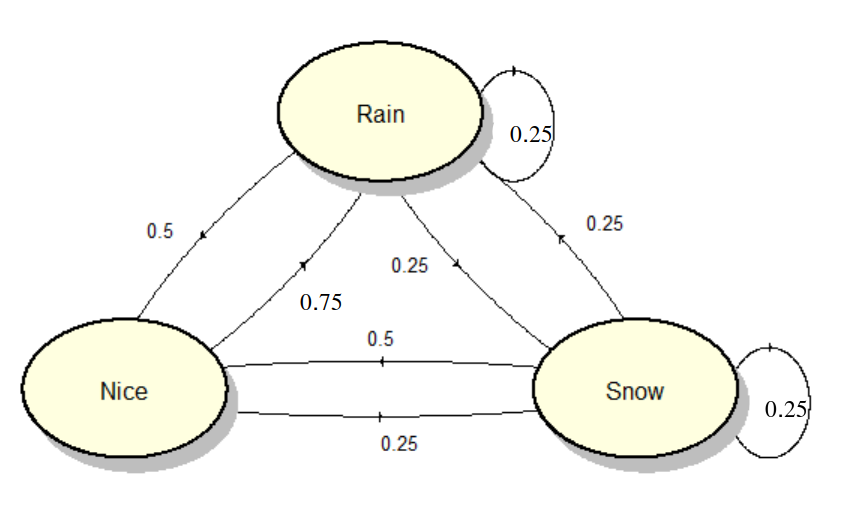
\includegraphics[scale=0.40]{Images/markovChain.png}
\end{figure}

En este caso modelamos el tiempo que hace en un día determinado
usando una Cadena de Márkov, donde los tres estados posibles son
`Lluvia', `Buen tiempo' y `Nieve'. Las ponderaciones entre
las flechas que conectan los estados representan la probabilidad
de, estando cierto día en el estado desde el que sale 
la flecha, que al día siguiente se pase al estado al que
llega la flecha. A estas probabilidades las llamaremos
`probabilidades de transición'.

Presentamos ahora, con un ejemplo similar, los Modelos Ocultos
de Márkov y el concepto de probabilidad de emisión.

\newpage
Consideremos el siguiente modelo de Márkov que también representa el tiempo en un día determinado, pero donde hemos considerado solos dos estados posibles `Rainy' y `Sunny'. Además hemos
añadido dos consecuencias posibles sobre el estado
de ánimo de algún sujeto particular, María, durante un día en función únicamente del tiempo de ese día, con las probabilidades indicadas
en las flechas de que el sujeto esté feliz `Happy' o 
molesto `Grumpy'.


\begin{figure}[H]
    \centering
    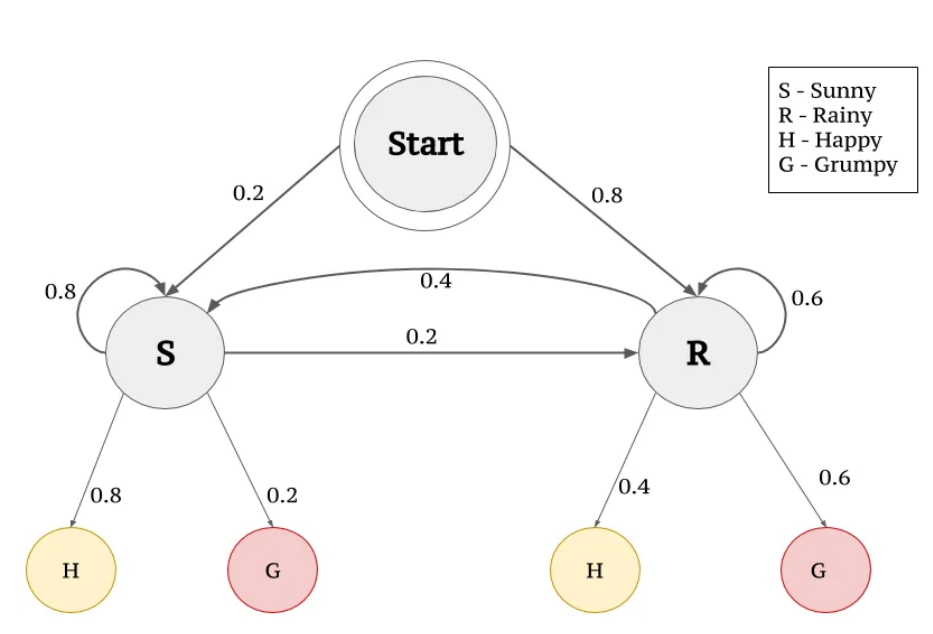
\includegraphics[scale=0.40]{Images/hmm.png}
\end{figure}

Bien, proponemos ahora la siguente situación:

\medskip
`María se ha mudado a Chile y no tenemos acceso a información sobre la meteorología del país por ninguna fuente. Sin embargo, por su manera
de comunicarse con nosotros, notamos que María ha estado
molesta durante tres días consecutivos.'
\medskip

Recordando que el estado de ánimo de María depende únicamente
del tiempo que hace en Chile, y que cuando hace sol tiene
un 80\% de probabilidad de estar contenta y un 20\% de estar molesta, mientras que cuando llueve las probabilidades son de un 0.4\% y de un 0.6\%. Planteamos la siguiente pregunta: ¿No es más
coherente inferir que, en principio, es más probable que
halla estado lloviendo en Chile estos tres días? 

Pues bien, nuestro propósito, y la cuestión que nos orientará
hacia el uso del algoritmo de Viterbi, es, tan solo teniendo
acceso a las consecuencias observables (en este caso, los estados de ánimo de María), tratar de inferir cuál es la secuencia
de estados en la cadena de Márkov que los ha producido.

Antes de proponer un abordaje rudimentario a este problema,
introduzcamos algo de terminología general sobre él.
Los fenómenos observables dentro del modelo son llamados \textbf{estados observados}, y los estados de la cadena de Márkov a los
que no tenemos acceso y que queremos adivinar son los \textbf{estados ocultos}. Un cierto estado oculto tiene una cierta
probabilidad de producir un determinado estado observado: la \textbf{probabilidad de emisión}. En nuestro ejemplo, la probabilidad de emisión del estado ``Happy" de María inducida por el 
estado oculto ``Sunny" de la cadena de Márkov es de $0.8$.

\medskip

Pues bien, notemos que las probabilidades que queremos calcular,
y de cual queremos extraer la más alta para saber cuál es la
hipótesis más probable son:

\begin{align*}
    P(G_1 \cap  G_2 \cap G_3 &\cap R_1 \cap  R_2 \cap R_3) \\
    P(G_1 \cap G_2 \cap G_3 &\cap R_1 \cap R_2 \cap S_3) \\
    P(G_1 \cap G_2 \cap G_3 &\cap R_1 \cap S_2 \cap R_3) \\
    P(G_1 \cap G_2 \cap G_3 &\cap R_1 \cap S_2 \cap S_3) \\
			    &\ldots \\
    P(G_1 \cap G_2 \cap G_3 &\cap S_1 \cap S_2 \cap S_3) \\
\end{align*} 

\text{Donde los subíndices representan cada uno
 de los tres días o etapas del proceso de Márkov}\\

Es decir, la probabilidad de que el causante del estado
observado haya sido cada una de las posibles secuencias de
estados ocultos posibles. Es claro que la mayor de estras probabilidades vendrá dada por el estado oculto que más probablemente
haya causado la secuencia de estados observados, y entonces
bastaría hacer estos cálculos para tener resuelto nuestro 
problema.
Sin embargo, nos encontramos con un impedimento: la eficiencia.
Veamos cómo calcularíamos una de estas probabilidades, por ejemplo la primera y aprovechemos para ver cómo las propiedades
de las cadenas de Márkov simplifican mucho el problema.

\begin{multline*}
    P(G_1 \cap  G_2 \cap G_3 \cap R_1 \cap  R_2 \cap R_3) = P(R_1 \mid \text{ Start }) \cdot  P(R_2  \mid R_1) \cdot  P(R_3  \mid  R_1 \cap R_2) \cdot P(G_1  \mid R_1 \cap R_2 \cap R_3)  
    \cdot \\ P(  G_2 \mid  G_1  \cap  R_1 \cap R_2 \cap R_3) \cdot P(  G_3 \mid  G_2 \cap G_1  \cap  R_1 \cap R_2 \cap R_3) 
\end{multline*} 

Ahora bien, usando que un estado en la cadena de Márkov depende
\textbf{únicamente del estado anterior}:

\begin{multline*}
    P(G_1 \cap  G_2 \cap G_3 \cap R_1 \cap  R_2 \cap R_3) = P(R_1 \mid \text{ Start }) \cdot  P(R_2  \mid R_1) \cdot  P(R_3  \mid R_2) \cdot P(G_1  \mid R_1)  
    \cdot \\ P(  G_2 \mid R_2) \cdot P(  G_3  \mid  R_3) 
\end{multline*} 

Pero en cualquier caso, teniendo en cuenta que en una
situación con $k$ estados posibles del proceso de Márkov y
$n$ observaciones tendríamos que efectuar $k^{n}$ cálculos de 
probabilidades como esta, notamos que el problema es del orden
$O(k^{n})$ con respecto al número de observaciones, y muy 
rápidamente los costes computacionales resultan inasumibles:
necesitamos de una herramienta que nos permita llegar
a esa combinación de estados ocultos que nos proporciona la probabilidad máxima de manera más eficiente. Aquí entra el algoritmo de Viterbi.

\newpage
\section{Definición del Algoritmo}

La idea detrás del algoritmo de Viterbi reside tras la
propiedad de subestructuras optimales de la que gozan las 
soluciones a los problemas que aborda. Y es que notemos que
una solución puede interpretarse como nada más que un
recorrido por etapas entre los distintos estados ocultos, de esta manera:

\vspace{0.5cm}

\begin{comment}
    \begin{figure}[H]
    \centering
    \includegraphics[scale=0.40]{Images/primera.jpeg}
    \end{figure}
\end{comment}

\begin{tikzpicture}[node distance={45mm}, thick, -stealth, font=\Huge, main/.style = {draw, circle}]
  
    \node[main] (O) {Start};
    \node[main] (S1) [above right of=O] {S};
    \node[main] (S2) [right of=S1] {S};
    \node[main] (S3) [right of=S2] {S};
    \node[main] (R1) [below right of=O] {R};
    \node[main] (R2) [right of=R1] {R};
    \node[main] (R3) [right of=R2] {R};

    \draw[-stealth] (O) -- node[font=\scriptsize, midway, above, sloped, pos=0.5] {$\textcolor{blue}{1} \times \textcolor{green}{0.2} \times \textcolor{red}{0.2} = 0.4$} (S1);
    \draw[-stealth] (O) -- node[font=\scriptsize, midway, above, sloped, pos=0.5] {$\textcolor{blue}{1} \times \textcolor{green}{0.8} \times \textcolor{red}{0.6} = 0.48$} (R1);
    \draw[-stealth] (S1) -- node[font=\scriptsize, midway, above, sloped, pos=0.5] {$\textcolor{blue}{0.04} \times \textcolor{green}{0.8} \times \textcolor{red}{0.2} = 0.4$} (S2);
    \draw[-stealth] (S1) -- node[font=\scriptsize, midway, above, sloped, pos=0.25] {$\textcolor{blue}{0.04} \times \textcolor{green}{0.2} \times \textcolor{red}{0.6} = 0.0048$} (R2);
    \draw[-stealth] (R1) -- node[font=\scriptsize, midway, above, sloped, pos=0.25] {$\textcolor{blue}{0.48} \times \textcolor{green}{0.4} \times \textcolor{red}{0.2} = \textbf{0.0384}$} (S2);
    \draw[-stealth] (R1) -- node[font=\scriptsize, midway, above, sloped, pos = 0.5] {$\textcolor{blue}{0.48} \times \textcolor{green}{0.6} \times \textcolor{red}{0.6} = \textbf{0.288}$} (R2);
    \draw[-stealth] (S2) -- (S3);
    \draw[-stealth] (S2) -- (R3);
    \draw[-stealth] (R2) -- (R3);
    \draw[-stealth] (R2) -- (S3);

\end{tikzpicture}

\vspace{0.5cm}

En esencia, podemos ver que considerando cada estado como un nodo siempre
obtenemos una estrucutura de grafo donde los nodos se organizan por 
columnas (cada columna hará referencia a una etapa) y cada nodo (estado)
solo podrá conectarse con algún nodo de las columnas adyacences (referiendose
a la transición de estados). Notemos que partiendo de un estado
solo tiene sentido cambiar a otro estado cuando pasemos a otra etapa, así
los nodos(estados) nunca pueden estar conectados con nodos que sean de 
la misma columna, puesto que no se considera la transición de estados 
en una misma etapa. 

En cada estado oculto hemos calculado, usando los datos del diagrama,
la probabilidad de que éste haya sido el causante del estado
de ánimo de María (`Grumpy') en cada día. Notemos que al
pasar de una etapa a otra lo único que hacemos es multiplicar
la probabilidad de estar en el estado anterior por la probabilidad de transición al estado al que llegamos y por la probabilidad
de emisión del estado observado `Grumpy' en cada caso ($0.2$ si
el estado oculto es `Sunny' y $0.6$ si el estado oculto
es `Rainy'). Se han marcado en cada paso en verde la \textcolor{green}{probabilidad
de transición} y en rojo la \textcolor{red}{probabilidad de emisión} del estado
que hemos observado. También, para los estados ocultos
de la segunda etapa, se han encuadrado las probabilidades
acumuladas máximas al llegar a ese estado de entre las dos
posibles que hay: considerar la diferencia entre las probabilidades de llegada por diferentes caminos será fundamental
más adelante.

De esta forma, vemos ya que nuestro problema, bajo este planteamiento, queda sintetizado en encontrar cuál es la secuencia
de estados que tiene mayor probabilidad acumulada al llegar a la última de las 3 etapas del diagrama (una suerte maximización
en el cálculo de caminos). 

\medskip

Estamos ya en condiciones de presentar la idea clave del algoritmo de Viterbi, que nos permite en cada paso descartar como
imposibles ciertos caminos (secuencias de estados ocultos) en
tanto que no podrán llevarnos a la secuencia con mayor
probabilidad al final del diagrama, que es la que nos interesa.

Para ello, observemos la probabilidad de subestructuras
optimales de una solución al problema de optimización frente
al que nos encontramos. Dado un camino óptimo de la primera
a la quinta etapa en un problema análogo al ejemplo que venimos siguiendo, partámosla por la tercera, y consideremos
los dos caminos que nos quedan a la derecha y a la izquierda
(de la primera a la tercera etapa y de la tercera a la quinta
respectivamente).

La idea queda clara con una imagen:

\begin{comment}
    \begin{figure}[H]
	    \centering
	    \includegraphics[scale=0.40]{Images/segunda.jpeg}
    \end{figure}
\end{comment}

\begin{tikzpicture}[node distance={30mm}, thick, -stealth, font=\huge, main/.style = {draw, circle}]
    \node[main] (S1) {S};
    \node[main] (S2) [right of=S1] {S};
    \node[main] (S3) [right of=S2] {S};
    \node[main] (S4) [right of=S3] {S};
    \node[main] (S5) [right of=S4] {S};
    \node[main] (R1) [below of=S1] {R};
    \node[main] (R2) [right of=R1] {R};
    \node[main] (R3) [right of=R2] {R};
    \node[main] (R4) [right of=R3] {R};
    \node[main] (R5) [right of=R4] {R};

    \node[main] (1) [font=\small] at ($(S1) + (0, 15mm)$) {1};
    \node[main] (2) [font=\small] at ($(S2) + (0, 15mm)$) {2};
    \node[main] (3) [font=\small] at ($(S3) + (0, 15mm)$) {3};
    \node[main] (4) [font=\small] at ($(S4) + (0, 15mm)$) {4};
    \node[main] (5) [font=\small] at ($(S5) + (0, 15mm)$) {5};
    
    \node[main] (I1) [coordinate] at ($(3) + (0, 8mm)$) {};
    \node[main] (I2) [coordinate] at ($(R3) + (0, -10mm)$) {};

    \draw[dotted] (I1) -- (I2);
    
    \draw[-stealth] (S1) -- (S2);
    \draw[-stealth] (S2) -- (S3);
    \draw[-stealth] (S3) -- (S4);
    \draw[-stealth] (S4) -- (S5);
    
    \draw[-stealth] (R1) -- (R2);
    \draw[-stealth] (R2) -- (R3);
    \draw[-stealth] (R3) -- (R4);
    \draw[-stealth, color=green, ultra thick] (R4) -- (R5);
    
    \draw[-stealth, color=green, ultra thick] (S1) -- (R2);
    \draw[-stealth] (S2) -- (R3);
    \draw[-stealth, color=green, ultra thick] (S3) -- (R4);
    \draw[-stealth] (S4) -- (R5);
    
    \draw[-stealth] (R1) -- (S2);
    \draw[-stealth, color=green, ultra thick] (R2) -- (S3);
    \draw[-stealth] (R3) -- (S4);
    \draw[-stealth] (R4) -- (S5);
    
    
\end{tikzpicture}

\vspace{0.5cm}

Es claro que, por ejemplo, el sub-camino derecho es la forma
óptima (con mayor probabilidad acumulada) de llegar de la tercera a la quinta etapa, porque de ser otro 
el camino óptimo para ir de la tercera a la quinta etapa, tendríamos que podríamos formar un 
camino mejor que nuestra solución (total) original uniendo el camino de la parte izquierda 
(de la etapa 1 a la etapa 3) de nuestra solución original
con el camino óptimo de la etapa 3 a la etapa 5
y tendríamos una contradicción
con nuestra suposición de que partíamos de un camino óptimo
de \textbf{1} a \textbf{5}. Por tanto, sabemos
que cualquier solución que propongamos que pase por \textbf{S} en la etapa \textbf{3}, para intentar ser óptima, no puede más
que hacer exactamente el camino marcado en verde hasta la última
etapa.

Consideremos ahora que queremos construir una solución
óptima pero tan solo sabemos la existencia del camino óptimo
de \textbf{3} a \textbf{5} anterior.

\begin{comment}
    \begin{figure}[H]
    \centering
    \includegraphics[scale=0.40]{Images/adivinar.jpeg}
    \end{figure}
\end{comment}

\begin{tikzpicture}[node distance={30mm}, thick, -stealth, font=\huge, main/.style = {draw, circle}]
    \node[main] (S1) {S};
    \node[main] (S2) [right of=S1] {S};
    \node[main] (S3) [right of=S2] {S};
    \node[main] (S4) [right of=S3] {S};
    \node[main] (S5) [right of=S4] {S};
    \node[main] (R1) [below of=S1] {R};
    \node[main] (R2) [right of=R1] {R};
    \node[main] (R3) [right of=R2] {R};
    \node[main] (R4) [right of=R3] {R};
    \node[main] (R5) [right of=R4] {R};

    \node[main] (1) [font=\small] at ($(S1) + (0, 15mm)$) {1};
    \node[main] (2) [font=\small] at ($(S2) + (0, 15mm)$) {2};
    \node[main] (3) [font=\small] at ($(S3) + (0, 15mm)$) {3};
    \node[main] (4) [font=\small] at ($(S4) + (0, 15mm)$) {4};
    \node[main] (5) [font=\small] at ($(S5) + (0, 15mm)$) {5};

    \node[main] (I1) [coordinate] at ($(3) + (0, 8mm)$) {};
    \node[main] (I2) [coordinate] at ($(R3) + (0, -15mm)$) {};

    \node[main] (I3) [coordinate] at ($(S3) + (7mm, 7mm)$) {};
    \node[main] (I4) [coordinate] at ($(R3) + (7mm, -7mm)$) {};
    \node[main] (I5) [coordinate] at ($(S1) + (-7mm, 7mm)$) {};
    \node[main] (I6) [coordinate] at ($(R1) + (-7mm, -7mm)$) {};

    \draw[dotted] (I1) -- (I2);
    
    \draw[dotted, color=blue] (I3) -- (I4);
    \draw[dotted, color=blue] (I3) -- (I5);
    \draw[dotted, color=blue] (I5) -- (I6);
    \draw[dotted, color=blue] (I4) -- (I6);

    \draw[-stealth] (S1) -- (S2);
    \draw[-stealth] (S2) -- (S3);
    \draw[-stealth] (S3) -- (S4);
    \draw[-stealth] (S4) -- (S5);
    
    \draw[-stealth] (R1) -- (R2);
    \draw[-stealth] (R2) -- (R3);
    \draw[-stealth] (R3) -- (R4);
    \draw[-stealth, color=red, ultra thick] (R4) -- (R5);
    
    \draw[-stealth, color=green, ultra thick] (S1) -- (R2);
    \draw[-stealth] (S2) -- (R3);
    \draw[-stealth, color=red, ultra thick] (S3) -- (R4);
    \draw[-stealth] (S4) -- (R5);
    
    \draw[-stealth] (R1) -- (S2);
    \draw[-stealth, color=green, ultra thick] (R2) -- (S3);
    \draw[-stealth] (R3) -- (S4);
    \draw[-stealth] (R4) -- (S5);
    
    
\end{tikzpicture}

\vspace{0.5cm}


Entonces, para encontrarla, estamos considerando cuáles de los caminos para llegar desde el comienzo hasta
\textbf{S} en la etapa \textbf{3} es el que logra mayor probabilidad acumulada. Los caminos posibles son los siguientes:
\begin{itemize}
    \item $S_1 \to S_2 \to S_3$ 
    \item $S_1 \to R_2 \to S_3$ 
    \item $R_1 \to S_2 \to S_3$ 
    \item $R_1 \to R_2 \to S_3$ 
\end{itemize}

Entonces, notemos que solo tenemos que continuar considerando uno de los 4 caminos anteriores, el que tenga
mayor probabilidad acumulada al llegar hasta $S_3$, porque desde
ese punto lo único que harán los caminos será seguir \textbf{todos el mismo} camino óptimo
que existe (aunque no lo conociésemos como en este caso) desde 
$S_3$ hasta $R_5$, y ya que para recorrer
ese camino se avanzará multiplicando por unas cantidades
fijas (las probabilidades de emsión y transición), será ese el que llegará al final
con mayor probabilidad acumulada. Por tanto, podemos
dejar de extender cualquier otro de los 4, pues no aspiran
a ser la solución de nuestro problema.

De esta forma, en general, y aquí está \textbf{la clave} del 
Algoritmo de Viterbi, al llegar a cualquier nodo dentro
del diagrama de estados ocultos que estamos recorriendo\footnote{multiplicando por probabilidades de transición y 
por probabilidades de emisión de estados observados en cada paso
para encontrar el camino de probabilidad máxima} tan solo
tenemos que continuar (seguir calculando posibilidades) el
camino que tenga mayor probabilidad acumulada de entre todos
los que intersecan en ese nodo. Y esto es por la razón recién vista: todo camino que parta de ese nodo y aspire a ser la solución óptima, seguirá el mismo camino máximo (siempre existente, aunque fuera desconocido) desde ese nodo hasta el final del diagrama, pudiendo entonces ser solución óptima solo
el camino que tenga mayor probabilidad acumulada en el 
momento de la intersección.

\medskip

Estamos ya en condiciones, por tanto, de presentar
la recurrencia que define el Algoritmo de Viterbi: determinar 
la máxima probabilidad de encontrarnos en un estado oculto $s$ en la observación $t$-ésima (de entre todas las posibles
secuencias de estados ocultos que pudieran habernos
llevado a esa observación). De forma rudimentaria y quizá
para algunos más clara: `de entre todas las posibles secuencias
de estados que desencadenan en el estado observado en la etapa
$t$-ésima, consideramos cuál es la probabilidad que tiene
aquella que más probabilidad tiene'.

Siendo $S$ el conjunto de estados ocultos, $\pi_{s} \text{ y }a_{r,s}$ las probabilidades iniciales y de transición respectivamente y $b_{s,o}$ la probabilidad de emisión de la observación
$o$ en el estado $s$,  y 
teniendo una secuencia de $T$ observaciones $o_0,o_1, \ldots , o_{T-1}$, nos definimos dos matrices de tamaño $T \times \left|S\right|$ de la siguiente manera:

\begin{equation*}
    P_{t,s} =
    \begin{cases}
	\pi_s \cdot b_{s,o_t} & \text{if } t=0, \\
	\max_{r \in S} \left(P_{t-1,r} \cdot a_{r,s} \cdot b_{s,o_t} \right) & \text{if } t>0.
    \end{cases}
\end{equation*} 
\begin{equation*}
    Q_{t,s} =
    \begin{cases}
	-1 & \text{ if } t = 0, \\
	\text{arg}\max_{r \in S} \left(P_{t-1,r} \cdot a_{r,s} \cdot b_{s,o_t} \right) & \text{if } t>0.
    \end{cases}
\end{equation*} 

Donde en la matriz $P$ guardamos las probabilidades ya explicadas (notemos que la toma de la probabilidad máxima en cada nodo
es exactamente la poda de caminos posibles que se ha explicado
anterioremente) y en la matriz $Q$ guardamos simplemente
en cada estado oculto al que llegamos, cuál es el estado
desde el que llegamos, y que nos servirá para la reconstrucción
del camino de probabilidad acumulada máxima al final del
algoritmo. 

Nótese que es ya totalmente claro que en el núcleo del Algoritmo de Viterbi residen las ideas de la programación dinámica:
el principio de Optimalidad de Bellman sobre la suboptimalidad
de particiones de una solución, y la reducción de la información para quedarnos tan solo con la relevante en cada caso (no nos
interesa por qué camino hemos llegado a cierto estado oculto para tomar una decisión sobre el siguiente, sino tan solo cuál es la probabilidad acumulada al llegar hasta él). También esto
se manifiesta en el carácter iterativo del algoritmo para
rellenar la tabla de probabilidades que nos da finalmente
la solución y la forma de reconstruir el camino, como podemos
ver en la siguiente propuesta de pseudocódigo:

\begin{minipage}{0.9\textwidth}
\begin{verbatim}
    transProb <-- S x S transition probability matrix
    emitProb <--- S x K emission probability matrix (K states of the observations)
    obs <-- array of T observations

    func Viterbi(states, initProb, transProb, emitProb, obs)
        prob <-- T x S matrix of 0's
        prev <-- T x S matrix of -1's

        // Inicializamos la probabilidad
        // de las primeras observaciones en los
        // primeros estados
        for each state s in states do
            prob[0][s] = init[s] * emit[s][obs[0]]
	
        // Para cada etapa t, guardamos
        // la probabilidad de alcanzar el estado 
        // s considerando la máxima probabilidad 
        // acumulada con la que se pueda llegar a
        // s desde cualquier nodo r
        for (t = 1; t < T; ++t) 
            for each state r in states do
                for each state s in states do
                    newProb = prob[t-1][r] * trans[r][s] *
                              emit[s][obs[t]]
                    if newProb > prob[t][s]
                        prob[t][s] = newProb
                        prev[t][s] = r
	

        // Reconstruimos, metiendo como estado final
        // del camino aquel que termine con probabilidad
        // acumulada mayor
        path <-- empty array of size T
        path[T-1] <-- argmax_s (prob[T-1][s])

        // Y cada paso será el previo del siguiente
        for (t = T - 2; t >= 0)
            path[t] = prev[t+1][path[t+1]] 
\end{verbatim}
\end{minipage}

\medskip

Notamos que, siendo clara la eficacia del algoritmo, 
obtenemos una eficiencia abrumadoramente mejor que en 
el cálculo por fuerza bruta, el particular, 
del orden de $O(T \times \left|S\right|^{2})$

\newpage

\section{Ejemplos de uso}

\subsection{Cálculo de caminos mínimos por etapas}

Veamos ahora cómo se usa el algoritmo de Viterbi para el cálculo de caminos mínimos 
entre dos nodos en un grafo mediano (Lattice Gragh)
\footnote{Un grafo mediano en Matemáticas es un grafo no dirigido en que 
cualesquiera tres nodos a, b, y c tienen un único mediano. Un mediano (de a, b y c) es un nodo 
que pertenece a los caminos más cortos entre cualquier par de nodos a,b y c.}
donde además se exige que los nodos estén organizados por columnas 
y que cada nodo solo se pueda conectar con los nodos de las columnas vecinas adyacentes, es decir, no está permitido que se conecten nodos de una misma columna y tampoco nodos que no estén en columnas adyacentes. Este camino buscado también es llamado camino de Viterbi (\emph{Viterbi path}).

\begin{figure}[!hbt]
    \centering
    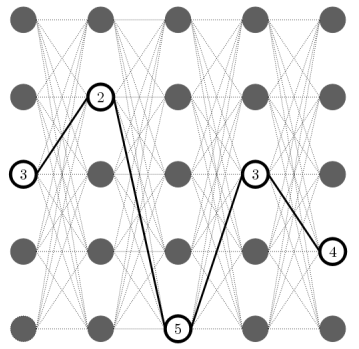
\includegraphics[scale=0.5]{Images/IntroViterbi.png}
    \caption{Ejemplo de grafo con nodos organizados por columnas}
\end{figure}

Podemos ver que esta  estructura coincide con la de los grafos que usamos para representar las cadenas de sucesos 
modelados con un Modelo de Markov. 

Aplicándolo a nuestro problema notemos que dado un grafo de este estilo, y dos nodos \textit{start} y \textit{end}, en nuestro problema no es restrictivo 
considerar única y exclusivamente las columnas comprendidas entre dichos dos nodos, y además, podemos 
ignorar el resto de nodos de las respectivas columnas a las que pertenecen dichos nodos
\textit{start} y \textit{end}. También, está claro que debido a la estructura, para llegar de un 
nodo a otro necesariamente tenemos que pasar por cada una de las columnas entre medias una vez. 

Teniendo en cuenta todo lo anterior, una forma sencilla de encontrar el camino sería 
listar todas los posibles caminos y quedarnos con el de mínimo coste, pero lo descartamos 
directamente por la ineficiencia, análogo razonamiento 
al realizado en la introducción. Aquí ya notamos la similitud con el ejemplo de la introducción. 

Vamos ahora a desarrollar el razonamiento a partir de un ejemplo con pocos nodos (en la figura hemos
obviado algunos caminos por limpieza): 

\begin{figure}[!hbt]
    \centering
    \begin{tikzpicture}[
        -stealth, auto, node distance=3cm,
        thick, main node/.style={circle, draw}
    ]
    
    \node[main node] (S) {Start};
    \node[main node] (A1) at ($(S) + (3, 2)$) {$A_1$};
    \node[main node] (A2) at ($(S) + (3, 0)$) {$A_2$};
    \node[main node] (A3) at ($(S) + (3, -2)$) {$A_3$};
    \node[main node] (B1) at ($(A1) + (3, 0)$) {$B_1$};
    \node[main node] (B2) at ($(A2) + (3, 0)$) {$B_2$};
    \node[main node] (B3) at ($(A3) + (3, 0)$) {$B_3$};
    \node[main node] (C1) at ($(B1) + (3, 0)$) {$C_1$};
    \node[main node] (C2) at ($(B2) + (3, 0)$) {$C_2$};
    \node[main node] (C3) at ($(B3) + (3, 0)$) {$C_3$};
    \node[main node] (E) [right of=C2] {End};
    
    \path
        (S) edge node [left] {6} (A1)
            edge node {1} (A2)
            edge node [left] {3} (A3)
        (A1) edge node {3} (B1)
        (A2) edge node {2} (B1)
        (A3) edge node [below] {9} (B1)
        (B1) edge (C1)
            edge (C2)
            edge (C3)
        (B2) edge (C1)
            edge (C2)
            edge (C3)
        (B3) edge (C1)
            edge (C2)
            edge (C3)
        (C1) edge (E)
        (C2) edge (E)
        (C3) edge (E);
    \end{tikzpicture}
    \caption{Ejemplo de grafo con nodos organizados por columnas}
\end{figure}

Por lo razonado anteriormente, como tenemos que pasar por cada una de las columnas A-B-C necesariamente, veamos con más detalle 
los primeros pasos.

De los caminos que empiezan en \textit{start} y llegan a los distintos nodos de A, a priori, no podemos concluir con qué 
cámino sería el óptimo a tomar pues los costes posteriores podrían influir en nuestra decisión final, 
pero si nos fijamos en los nueve caminos que conducen a los distintos nodos de la
columna B sí que podemos obtener información útil. 

\begin{figure}[!hbt]
    \centering
    \begin{tikzpicture}[
        -stealth, auto, node distance=3cm,
        thick, main node/.style={circle, draw}
    ]
    
    \node[main node] (S) {Start};
    \node[main node] (A1) at ($(S) + (3, 2)$) {$A_1$};
    \node[main node] (A2) at ($(S) + (3, 0)$) {$A_2$};
    \node[main node] (A3) at ($(S) + (3, -2)$) {$A_3$};
    \node[main node] (B1) at ($(A1) + (3, 0)$) {$B_1$};
    \node[main node] (B2) at ($(A2) + (3, 0)$) {$B_2$};
    \node[main node] (B3) at ($(A3) + (3, 0)$) {$B_3$};
    \node[main node] (C1) at ($(B1) + (3, 0)$) {$C_1$};
    \node[main node] (C2) at ($(B2) + (3, 0)$) {$C_2$};
    \node[main node] (C3) at ($(B3) + (3, 0)$) {$C_3$};
    \node[main node] (E) [right of=C2] {End};
    
    \path
        (S) edge node [left] {6} (A1)
            edge[red] node {1} (A2)
            edge node [left] {3} (A3)
        (A1) edge node {3} (B1)
        (A2) edge[red] node {2} (B1)
        (A3) edge node [below] {9} (B1)
        (B1) edge (C1)
            edge (C2)
            edge (C3)
        (B2) edge (C1)
            edge (C2)
            edge (C3)
        (B3) edge (C1)
            edge (C2)
            edge (C3)
        (C1) edge (E)
        (C2) edge (E)
        (C3) edge (E);
    \end{tikzpicture}
    \caption{Camino mínimo a los nodos de la columna B}
\end{figure}

Empecemos fijándonos en particular en el nodo $B_1$. Para llegar a 
$B_1$ nos encontramos con que existen tres caminos que conducen a $B_1$,
de estos tres sí que está claro qué cámino va a ser el óptimo a tomar para 
llegar a $B_1$, que en nuestro caso es la que pasa por $A_2$ (por ser el de coste mínimo). Por tanto,
el resto de posibles caminos a $B_1$ los podemos descartar y a partir de entonces 
sabemos que todos los caminos parciales que surjan de $B_1$ hasta \textit{end}, 
lo óptimo sería pasar por $A_2$.

Notemos también que la manera correcta de abordar los caminos 
ha de ser de $A\rightarrow B_i$ (forma a), en lugar de $A_k \rightarrow B$ (forma b).
La forma b no es concluyente, es por esto que cuando consideramos 
los caminos desde \textit{start} hasta los nodos de la columna A
no pudimos concluir con nada.

\begin{figure}[!hbt]
    \centering
    \begin{subfigure}[b]{0.45\textwidth}
    \centering
    \begin{tikzpicture}
        % Nodes
        \node[draw, circle] (A1) at (0,3) {$A_1$};
        \node[draw, circle] (A2) at (0,2) {$A_2$};
        \node[draw, circle] (A3) at (0,1) {$A_3$};
        \node[draw, circle] (An) at (0,0) {$A_n$};
    
        \node[draw, circle] (B1) at (2,3) {$B_1$};
        \node[draw, circle] (B2) at (2,2) {$B_2$};
        \node[draw, circle] (B3) at (2,1) {$B_3$};
        \node[draw, circle] (Bn) at (2,0) {$B_n$};
        
        % Arrows
        \draw[-stealth] (A1) -- (B1);
        \draw[-stealth] (A2) -- (B1);
        \draw[-stealth] (A3) -- (B1);
        \draw[-stealth] (An) -- (B1);
    \end{tikzpicture}
    \caption{Forma a, correcta.}
    \end{subfigure}
    \begin{subfigure}[b]{0.45\textwidth}
    \centering
    \begin{tikzpicture}
        % Nodes
        \node[draw, circle] (A1) at (0,3) {$A_1$};
        \node[draw, circle] (A2) at (0,2) {$A_2$};
        \node[draw, circle] (A3) at (0,1) {$A_3$};
        \node[draw, circle] (An) at (0,0) {$A_n$};
    
        \node[draw, circle] (B1) at (2,3) {$B_1$};
        \node[draw, circle] (B2) at (2,2) {$B_2$};
        \node[draw, circle] (B3) at (2,1) {$B_3$};
        \node[draw, circle] (Bn) at (2,0) {$B_n$};
        
        % Arrows
        \draw[-stealth] (A1) -- (B1);
        \draw[-stealth] (A1) -- (B2);
        \draw[-stealth] (A1) -- (B3);
        \draw[-stealth] (A1) -- (Bn);
    \end{tikzpicture}
    \caption{Forma b, incorrecta.}
    \end{subfigure}
\end{figure}

En resumen, extrapolando a casos de tamaño mayor concluimos que basta con ir calculando el cámino mínimo para los nodos 
intermediarios para ir descartando posibles cáminos que ya sabemos que no son el óptimo 
y así alcanzando el camino mínimo buscado. Así, vemos que sigue al pie de la letra la lógica bajo el Algoritmo de Viterbi, luego
es un caso válido donde se puede aplicar dicho algoritmo.
La ligera diferencia a lo explicado anteriormente con los estados ocultos modelados con los Modelos de Markov es que,
aquí tenemos costes de caminos a diferencia de probabilidades, pero 
en esencia siguen el mismo funcionamiento. Cuando seleccionamos un camino (buscando el camino de coste mínimo),
el coste de nuestro camino aumenta, al igual que cuando seleccionamos un nuevo estado (buscando la secuencia de estados
de mayor probabilidad), tenemos que multiplicar
nuestra probabilidad total acumulada por dicha probabilidad de cambio 
de estado, y por tanto, nuestra probabilidad
total disminuye. 

\myparagraph{Resolución del ejemplo: }

Ahora vamos a resolver el ejemplo anterior con el algoritmo de Viterbi dadas
ahora los costes de todos los caminos en las siguientes tablas:

\begin{table}[h!]
\centering

\begin{subtable}[t]{0.45\textwidth}
\centering
\begin{tabular}{|c|c|c|c|}
\hline
     & \textbf{A\textsubscript{1}} & \textbf{A\textsubscript{2}} & \textbf{A\textsubscript{3}} \\ \hline
\textbf{S}    & 6    & 1    & 3    \\ \hline
\textbf{B\textsubscript{1}} & 3    & 2    & 9    \\ \hline
\textbf{B\textsubscript{2}} & 5    & 4    & 1    \\ \hline
\textbf{B\textsubscript{3}} & 2    & 6    & 3    \\ \hline
\end{tabular}
\end{subtable}
\hspace{5mm}
\begin{subtable}[t]{0.45\textwidth}
\centering
\begin{tabular}{|c|c|c|c|}
\hline
     & \textbf{C\textsubscript{1}} & \textbf{C\textsubscript{2}} & \textbf{C\textsubscript{3}} \\ \hline
\textbf{E}    & 1    & 5    & 3    \\ \hline
\textbf{B\textsubscript{1}} & 2    & 3    & 1    \\ \hline
\textbf{B\textsubscript{2}} & 6    & 3    & 2    \\ \hline
\textbf{B\textsubscript{3}} & 2    & 3    & 3    \\ \hline
\end{tabular}
\end{subtable}
\end{table}

Mantendremos dos tablas para el algoritmo, uno para reconstruir el camino 
y otro para los costes. La primera columna representa la columna A, la segunda
la columna B y así sucesivamente hasta la última que representa el coste 
para llegar a \textit{end} desde nodos de la última columna de nodos.
Para cada posición (i,j), este hará referencia al nodo i-ésimo de la columna j-ésima, así, (1,1) representa al 
nodo $A_1$. En la tabla de costes, cada posición almacenará el coste 
mínimo para llegar desde \textit{start} hasta al nodo que representa. Y, en 
la tabla de caminos, cada casilla almacenará qué nodo de la columna anterior ha sido 
elegido, notemos que la primera columna se rellenará con un valor por defecto,
sease -1, para representar el nodo origen.

En la siguiente tabla se puede ver qué representa el valor de cada casilla,
donde notamos por $B \rightarrow C_1$ al coste (acumulado) o nodo previo (dependiendo de en que tabla estemos) correspondiente
al camino óptimo para ir desde la columna $B$ hasta el nodo $C_1$.

\begin{table}[!hbt]
\centering\begin{tabular}{|c|c|c|c|}
\hline
$S \rightarrow A_1$ & $A \rightarrow B_1$ & $B \rightarrow C_1$ & $C_1 \rightarrow E$ \\ \hline
$S \rightarrow A_2$ & $A \rightarrow B_2$ & $B \rightarrow C_2$ & $C_2 \rightarrow E$ \\ \hline
$S \rightarrow A_3$ & $A \rightarrow B_3$ & $B \rightarrow C_3$ & $C_3 \rightarrow E$ \\ \hline
\end{tabular}
\end{table}

Siguiendo los pasos explicados, cuando hayamos procesado/llegado al nodo $B_1$ tendremos: 

\begin{table}[h!]
\centering

\begin{subtable}[t]{0.45\textwidth}
\centering\begin{tabular}{|c|c|c|c|}
\hline
6 & 1+2 & - & - \\ \hline
1 & - & - & - \\ \hline
3 & - & - & - \\ \hline
\end{tabular}
\caption{Tabla de costes}
\end{subtable}
\hspace{5mm}
\begin{subtable}[t]{0.45\textwidth}
\centering
\begin{tabular}{|c|c|c|c|}
\hline
-1 & 2 & - & -\\ \hline
-1 & - & - & -\\ \hline
-1 & - & - & -\\ \hline
\end{tabular}
\caption{Tabla de caminos}
\end{subtable}
\end{table}

Obviando los pasos intermedios que son meros cálculos y comprobaciones obtenemos como resultado:

\begin{table}[h!]
\centering

\begin{subtable}[t]{0.45\textwidth}
\centering\begin{tabular}{|c|c|c|c|}
\hline
6 & 3 & 5 & 6 \\ \hline
1 & 4 & 6 & 11 \\ \hline
3 & 6 & 4 & 4 \\ \hline
\end{tabular}
\caption{Tabla de costes}
\end{subtable}
\hspace{5mm}
\begin{subtable}[t]{0.45\textwidth}
\centering
\begin{tabular}{|c|c|c|c|}
\hline
-1 & 2 & 1 & 1\\ \hline
-1 & 3 & 1 & 2\\ \hline
-1 & 3 & 1 & 3\\ \hline
\end{tabular}
\caption{Tabla de caminos}
\end{subtable}
\end{table}

De aquí sabemos que los costes mínimos a los nodos $B_j$, con $j \in {1,2,3}$, son de coste {3, 4, 6} y pasan por {$A_2, A_3, A_3$}, 
respectivamente. Para los nodos $C_k$, con $k \in {1,2,3}$, los costes mínimos son respectivamente {5, 6, 4} y pasando todos ellos por el 
nodo $B_1$. Finalmente, el coste mínimo de pasar por los nodos $C_k$ y llegar al nodo \textit{end} son
{6, 11, 4} respectivamente. Luego, el camino de coste mínimo tiene coste 4, y pasa por los nodos $C_3,\: B_1\: \text{y} \:A_2$, esto último se deduce 
naturalmente por la definición de la tabla de caminos. 

\subsection{\textit{`Part of Speech Tagging'}}

\myparagraph{Definición}

El Etiquetado Gramatical (en inglés, \textit{Part of Speech Tagging}) consiste en \textbf{clasificar} cada una de las palabras que aparecen en un discurso, en función tanto de su semántica como de su contexto en dicho discurso, tanto semántica como morfológicamente.

Esta tarea, que puede parecer un ejercicio de lenguaje para niños del colegio (y es que realmente lo es), tiene cierta complejidad a nivel computacional. \\

Por ejemplo, en castellano, la palabra \textit{para} en función del contexto podría ser una preposición o un verbo: no significa lo mismo (o al menos es poco probable) en las frases `para el tren' que en `para nosotros', igual que sucede con la palabra \textit{ratón}: no significa lo mismo (o al menos es poco probable) en las frases `se me estropeó el ratón' que en `el ratón se comió el queso'. En las frases anteriores tenemos \textbf{ambigüedad}, en el primer caso morfológica (la cual implica semántica), y en el segundo solo semántica. Nosotros nos centraremos en las morfológicas. Estas son más frecuentes en el inglés que en el castellano, motivo por el cual será el idioma de nuestro ejemplo. 

\myparagraph{Ejemplo ilustrativo}

En inglés, la siguiente frase presenta varias ambigüedades morfológicas:

\begin{center}
    The fans watch the race.
\end{center}

La palabra \textit{the} no presenta ninguna ambigüedad, siempre será un determinante. La palabra \textit{fans}, en función del contexto, puede ser un verbo (ventilar) o un nombre (ventilador, admirador), no obstante, sabemos que nunca será, por ejemplo, un determinante. Como ya hemos comentado obviaremos las ambigüedades semánticas. La palabra \textit{watch}, también podría ser un nombre (reloj) o un verbo (observar). Igualmente la palabra race podría tratarse de un nombre (carrera) o un verbo (correr, competir). 

\myparagraph{Definición del problema}

El problema entonces consiste en clasificar cada palabra (en nombre, verbo, determinante...) en función de su contexto del discurso y su propia semántica. Esto último hace referencia a que, dado un cierto tipo, habría palabras con mayor probabilidad de serlo que otras.

Como esta tarea la realizará un algoritmo y no una persona, no se podrá deducir el tipo con un 100\% de precisión, entonces lo que se pretende es dar la secuencia de tipos que se corresponda con el discurso con mayor probabilidad.

\myparagraph{Análisis del problema}

Para ello la primera idea clave es observar que el tipo de cada palabra está íntimamente relacionado con el tipo de la palabra que le precede\footnote{Aquí nos estamos basando solo en la palabra anterior, pero se podrían considerar las dos anteriores o incluso secuencias más largas.}. Por ejemplo, detrás de un determinante es muy probable que aparezca un nombre, e imposible que apareca un verbo. La otra idea es la que se comentó anteriormente, que para un determinado tipo, hay palabras que tendrían mayor probabilidad que otras de serlo. Por ejemplo, si una palabra fuese un verbo, sería imposible que fuese \textit{the}, y sería quizá más probable que fuese 
\textit{race} a que fuese \textit{fans}. \\

Estos datos, necesarios para la resolución del problema, se obtienen de forma empírica y hacen referencia a la \textbf{probabilidad de transición} y \textbf{probabilidad de emisión} que ya se ha comentado en el apartado de los modelos ocultos de Markov. \\

Las siguientes tablas muestran las probabilidades de transición y emisión que suponemos obtenidas de forma empírica (realmente se han rellenado de forma pseudoaleatoria, ya que lo que nos interesa es explicar el algoritmo):

\begin{table}[h!]
\centering
\caption{Probabilidades de Transición}
\begin{tabular}{|c|c|c|c|}
\hline
 & \textbf{Determinante} & \textbf{Nombre} & \textbf{Verbo} \\ \hline
\textbf{Inicio} & 0.8 & 0.2 & 0 \\ \hline
\textbf{Determinante} & 0 & 0.9 & 0.1 \\ \hline
\textbf{Nombre} & 0 & 0.5 & 0.5 \\ \hline
\textbf{Verbo} & 0.5 & 0.5 & 0 \\ \hline
\end{tabular}
\end{table}

% Tabla de Probabilidades de Emisión
\begin{table}[h!]
\centering
\caption{Probabilidades de Emisión}
\begin{tabular}{|c|c|c|c|c|c|}
\hline
     & \textbf{The} & \textbf{Fans} & \textbf{Watch} & \textbf{Race} \\ \hline
    \textbf{Determinante} & 0.2 & 0 & 0 & 0 \\ \hline
    \textbf{Nombre} & 0 & 0.1 & 0.3 & 0.1 \\ \hline
    \textbf{Verbo} & 0 & 0.2 & 0.15 & 0.3 \\ \hline
\end{tabular}
\end{table}

Algunos ejemplos para entender como se lee cada una de las tablas sería que la probabilidad de que haya un determinante al inicio es de 0.8, la de que vaya después de otro determinante o un nombre es 0, y de que vaya después de un verbo es 0.5. 

En la segunda tenemos que al encontrar un determinante hay una probabilidad de 0.2 de que sea \textit{the} y sin embargo es imposible que sea cualquiera de las otras 3 palabras. En esta tabla deberían aparecer más columnas, una por cada palabra que haya intervenido en los experimentos, de forma que las filas sumarían 1, aunque aquí solo hemos incluido las que intervienen en el discurso. La no ambigüedad de \textit{the} queda reflejada en que la probabilidad de que sea algo distinto de determinante (al menos para los tipos que hemos cogido) es 0. 

Insistimos en que estas tablas se han rellenado de forma pseudoaleatoria simulando que se han obtenido experimentalmente. \\

El diagrama de estados de este problema es el siguiente: \\

\begin{comment}
    \begin{figure}[H]
        \centering
        \includegraphics[trim=0cm 5cm 0cm 5cm, clip, width=\linewidth]{Images/POS-tag/estados.pdf}
        \caption{Diagrama de Estados del problema}
    \end{figure}
\end{comment}
\begin{figure}[H]
\begin{tikzpicture}[node distance={30mm}, thick, main/.style = {draw, circle}, sentence/.style = {draw}]

    \node[main] (O) {Start};
    \node[main] (D1) [right of=O] {Det};
    \node[main] (N1) [above right of=D1] {N};
    \node[main] (V1) [below right of=D1] {V};
    \node[main] (N2) [right of=N1] {N};
    \node[main] (V2) [right of=V1] {V};
    \node[main] (D2) [above right of=V2] {Det};
    \node[main] (N3) [above right of=D2] {N};
    \node[main] (V3) [below right of=D2] {V};
    
    \node[sentence] (2) at ($(N1) + (0, 10mm)$) {fans};
    \node[sentence] (1) at ($(D1) + (0, 10mm)$) {The};
    \node[sentence] (3) at ($(N2) + (0, 10mm)$) {watch};
    \node[sentence] (4) at ($(D2) + (0, 10mm)$) {the};
    \node[sentence] (5) at ($(N3) + (0, 10mm)$) {race};

    \draw[-stealth] (O) -- (D1);
    \draw[-stealth] (D1) -- (N1);
    \draw[-stealth] (D1) -- (V1);
    \draw[-stealth] (N1) -- (N2);
    \draw[-stealth] (N1) -- (V2);
    \draw[-stealth] (V1) -- (N2);
    \draw[-stealth] (V1) -- (V2);
    \draw[-stealth] (N2) -- (D2);
    \draw[-stealth] (V2) -- (D2);
    \draw[-stealth] (D2) -- (N3);
    \draw[-stealth] (D2) -- (V3);
\end{tikzpicture}
\caption{Diagrama de Estados del problema de Etiquetado Gramatical}
\end{figure}

Como vemos, tenemos un total de $1 \cdot 2 \cdot 2 \cdot 1 \cdot 2 = 8$ secuencias de estados posibles. Nuestro problema se reduce a estudiar cuál de nuestros estados tiene una mayor probabilidad. 

\myparagraph{Soluciones mejorables} 

Notemos que una solución siempre es calcular la probabilidad de cada estado y tomar la máxima al final (\textbf{fuerza bruta}). Si llamamos $P$ al número de tipos posibles de cada palabra (tomando máximo para la notación $O$) y $L$ a la longitud del discurso, vemos que la solución de fuerza bruta tendría una eficiencia de $O(P^L)$ por lo que crecería \textbf{exponencialmente} con la longitud del discurso y eso no interesa. Esta es la misma situación que ya vimos que se daba en los modelos de Markov (\ref{sec:markov-models}). \\

Otra solución, de eficiencia $O(L)$, sería simplemente para cada palabra tomar el tipo con mayor probabilidad. En este caso concreto, solo acertaríamos para el determinante \textit{the}, ya que diríamos que \textit{fans} es un verbo cuando es un nombre en este discurso, que \textit{watch} es un nombre cuando en el discurso es un verbo, y que \textit{race} es un verbo cuando en el discurso es un nombre.

\myparagraph{Solución con el algoritmo de Viterbi}

La solución que combina eficacia y eficiencia es la dada por el \textbf{algoritmo de Viterbi}, y es la que se describe a continuación: \\

Supongamos que, para todo $k$, con $0 \leq k \leq L$, $p_k$ denota el tipo morfológico de la palabra en la posición k-ésima, y $\omega_k$ representa la palabra que hay en dicha posición. Entonces, podremos escribir la probabilidad máxima del entre todos los estados ($S$) como:
\begin{equation}
    S = max_{p_i}\prod_{k=1}^LP(p_k|p_{k-1})\prod_{k=1}^LP(p_k|\omega_k)
    \label{eq:maxprobPOS-tagging}
\end{equation}

Donde P es la función de probabilidad. En la expresión de arriba el primer productorio hace referencia a las probabilidades de transmisión y el segundo a las probabilidades de emisión. 

En la siguiente figura se muestra la resolución del algoritmo para este ejemplo que se irá comentando paso a paso: \\

\begin{comment}
    \begin{figure}[H]
    \centering
    \includegraphics[trim=0cm 5cm 0.5cm 2cm, clip, width=\linewidth]{Images/POS-tag/resuelto2.pdf}
    \caption{Algoritmo de Viterbi sobre el Diagrama de Estados del problema}
    \end{figure}
\end{comment}
\begin{figure}[H]
\begin{tikzpicture}[node distance={33mm}, thick, -stealth, main/.style = {draw, circle}, sentence/.style = {draw}]

    \node[main] (O) {Start};
    \node[main] (D1) [right of=O] {Det};
    \node[main] (N1) [above right of=D1] {N};
    \node[main] (V1) [below right of=D1] {V};
    \node[main] (N2) [right of=N1] {N};
    \node[main] (V2) [right of=V1] {V};
    \node[main] (D2) [above right of=V2] {Det};
    \node[main] (N3) [above right of=D2] {N};
    \node[main] (V3) [below right of=D2] {V};
    
    \node[sentence] (2) at ($(N1) + (0, 10mm)$) {fans};
    \node[sentence] (1) at ($(D1) + (0, 13mm)$) {The};
    \node[sentence] (3) at ($(N2) + (0, 10mm)$) {watch};
    \node[sentence] (4) at ($(D2) + (0, 13mm)$) {the};
    \node[sentence] (5) at ($(N3) + (0, 10mm)$) {race};

    \draw[-stealth, color=green, ultra thick] (O) -- node[font=\tiny, midway, above, color=black] {$\textcolor{blue}{0.8} \times \textcolor{blue}{0.2} = 0.16$} (D1);
    \draw[-stealth, color=green, ultra thick] (O) -- node[font=\tiny, midway, below] {\textcolor{red}{[Det]}} (D1);
    \draw[-stealth, color=green, ultra thick] (D1) -- node[font=\tiny, midway, sloped, above, color=black] {$ \times \textcolor{blue}{0.9} \times \textcolor{blue}{0.1} = 0.0144$} (N1);
    \draw[-stealth, color=green, ultra thick] (D1) -- node[font=\tiny, midway, sloped, below, color=black] {\textcolor{red}{[Det, N]}} (N1);
    \draw[-stealth, color=green] (D1) -- node[font=\tiny, midway, sloped, above, color=black] {$\times \textcolor{blue}{0.9} \times \textcolor{blue}{0.1} = 0.0032$} (V1);
    \draw[-stealth, color=green] (D1) -- node[font=\tiny, midway, sloped, below, color=black] {\textcolor{red}{[Det, V]}} (V1);
    \draw[-stealth, color=green] (N1) -- node[font=\tiny, midway, sloped, above, color=black] {$\times \textcolor{blue}{0.5} \times \textcolor{blue}{0.3} = \textbf{0.00216}$} (N2);
    \draw[-stealth, color=green] (N1) -- node[font=\tiny, midway, sloped, below, color=black] {\textcolor{red}{[Det, N, N]}} (N2);
    \draw[-stealth, color=green, ultra thick] (N1) -- node[font=\tiny, midway, sloped, above, pos=0.25, color=black] {$\times \textcolor{blue}{0.5} \times \textcolor{blue}{0.15} = \textbf{0.0018}$} (V2);
    \draw[-stealth, color=green, ultra thick] (N1) -- node[font=\tiny, midway, sloped, below, pos=0.25, color=black] {\textcolor{red}{[Det, N, V]}} (V2);
    
    \draw[-stealth] (V1) -- node[font=\tiny, midway, sloped, above, pos=0.25] {$\times \textcolor{blue}{0.5} \times \textcolor{blue}{0.3} = 0.00048$} (N2);
    \draw[-stealth] (V1) -- node[font=\tiny, midway, sloped, above] {$\times \textcolor{blue}{0} = 0$} (V2);
    \draw[-stealth] (N2) -- node[font=\tiny, midway, sloped, above] {$\times \textcolor{blue}{0} = 0$} (D2);
    \draw[-stealth, color=green, ultra thick] (V2) -- node[font=\tiny, midway, sloped, below] {\textcolor{red}{[Det, N, V, Det]}} (D2);
    \draw[-stealth, color=green, ultra thick] (V2) -- node[font=\tiny, midway, sloped, above, color=black] {$\times \textcolor{blue}{0.5} \times \textcolor{blue}{0.2} = 0.000108$} (D2);
    \draw[-stealth, color=green, ultra thick] (D2) -- node[font=\tiny, midway, sloped, above, color=black] {$\times \textcolor{blue}{0.9} \times \textcolor{blue}{0.1} = \textbf{9.72} \cdot \textbf{10}^{\textbf{-6}}$} (N3);
    \draw[-stealth, color=green, ultra thick] (D2) -- node[font=\tiny, midway, sloped, below, color=black] {\textbf{\colorbox{yellow}{\textcolor{red}{[Det, N, V, Det, N]}}}} (N3);
    \draw[-stealth, color=green] (D2) -- node[font=\tiny, midway, sloped, above, color=black] {$\times \textcolor{blue}{0.1} \times \textcolor{blue}{0.3} = 3.24 \cdot 10^{-6}$} (V3);
    \draw[-stealth, color=green] (D2) -- node[font=\tiny, midway, sloped, below, color=black] {\textcolor{red}{[Det, N, V, Det, V]}} (V3);
\end{tikzpicture}
\caption{Algoritmo de Viterbi sobre el Diagrama de Estados del problema}
\end{figure}

Vamos a ir palabra por palabra, de forma que en cada una estaremos resolviendo el subproblema en el que el discurso llega hasta esa palabra. 

\myparagraph{Desarrollo del algoritmo}

\begin{enumerate}
    \item En la primera palabra, tenemos un único estado posible, el que la palabra \textit{the} sea un determinante. La probabilidad de este estado se calcula con la expresión anterior: la probabilidad de que la primera palabra sea un determinante (probabilidad de transición) por la probabilidad de que, siendo un determinante, que sea \textit{the} (probabilidad de emisión). Esto es $0.8 \cdot 0.2 = 0.16$.
    \item Para la segunda palabra, ya tenemos dos posibilidades: la primera que esta sea un nombre y la segunda, que sea un verbo. La primera se calcula como la probabilidad de que sea un nombre condicionada a que la palabra anterior es un determinante por la probabilidad de que la palabra sea fans, sabiendo que es un nombre. La segunda es análoga. Multiplicando las probabilidades por la que habíamos obtenido en el paso anterior, salen $0.16 \cdot 0.9 \cdot 0.1 = 0.0144$ para la primera y $0.16 \cdot 0.1 \cdot 0.2 = 0.0032$ para la segunda, obteniendo hasta ahora 2 ramas. Notemos que, obedeciendo al productorio de (\ref{eq:maxprobPOS-tagging}) tenemos que las probabilidades que vamos calculando son \textbf{acumuladas}, y por tanto, con respecto a la palabra anterior, \textbf{decrecientes} (cuanto más largo sea el discurso, más improbable será una secuencia de estados determinada).
    \item Para la tercera palabra, como tenemos 2 ramas activas y 2 posibilidades, tendremos 4 probabilidades a calcular. Para el estado N, tendremos la probabilidad de la secuencia [Det,N,N] que es 0.00216 y la de [Det,V,N] que es 0.00048. De estas dos posibilidades, se toma la máxima, descartando la rama [Det,V,N], ya que se sabe por el \textbf{principio de optimalidad de Bellman} que no va a dar con la solución óptima. Para el otro estado (V) de la palabra \textit{watch} se hace exactamente lo mismo, quedándonos con 2 ramas activas.
    \item En la cuarta palabra convergen ambas ramas activas y se calcula la probabilidad acumulada por cada una de ellas de la misma forma, tomando la máxima que es 0,000108.
    \item En la última palabra se separa la rama que teníamos en 2 posibles estados. Tomando de entre ellos la máxima probabilidad ya tendríamos la solución, que es [Det,N,V,Det,N] con una probabilidad de $9.72 \cdot 10^{-6}$, una probabilidad muy baja, pero la máxima de todas las combinaciones.
\end{enumerate}

El \textbf{paso clave} lo hemos desarrollado en el punto 3, que es donde se ve que el algoritmo de Viterbi mejora la fuerza bruta al descartar combinaciones sin llegar a procesarlas por completo.

Además podemos observar que la secuencia más probable del algoritmo de Viterbi coincide justo con la solución al ejemplo. 

\myparagraph{Comparación de eficiencia}

Por último veamos la eficiencia del algoritmo, comparándola con la fuerza bruta: 
En el desarrollo del algoritmo, para cada palabra, y para cada estado posible de la palabra evaluamos la probabilidad de dicho estado desde cada uno de los estados anteriores. Por ejemplo, para la tercera palabra, hemos evaluado la probabilidad de [Det,N,N] y [Det,V,N] para tomar máximo entre ambas, y la probabilidad de [Det,N,V] y [Det,V,V] para también tomar máximo entre ambas. En total en cada palabra evaluaremos $P^2$ probabilidades (P es el número de estados posibles de la palabra actual, y también el de los estados posibles de la palabra anterior, recordando que tomamos máximo para la notación $O$). Por tanto concluimos que este algoritmo tiene eficiencia $O(LP^2)$, por lo que el tiempo de cálculo crece \textbf{linealmente} respecto al número de palabras del discurso y se ve claramente la mejora en eficiencia respecto a la solución de fuerza bruta que era exponencial.

\newpage

\section{Conclusiones}

Con la realización de esta práctica, hemos visto ampliamente reforzados nuestros conocimientos sobre \textbf{Programación Dinámica}, aunque sea con un enfoque más centrado en el diseño de algoritmos y no tanto en la implementación de estos, con un ejemplo de algoritmo sencillo y famoso como es el \textbf{Algoritmo de Viterbi}. Hemos aprendido también un tema de grafos interesante como es el de las Cadenas de Markov y los Modelos Ocultos de Markov, así como su estrecha relación con el mencionado algoritmo y la utilidad de este último en áreas muy importantes de la \textbf{Inteligencia Artificial} como pueden ser el cálculo de caminos mínimos por etapas y incluso el etiquetado gramatical, próximo a la predicción de palabras y estudio computacional del lenguaje natural. \\

Además, hemos tenido que realizar un \textbf{trabajo de investigación} para saber de qué se trataba el algoritmo de Viterbi así como informarnos acerca de dónde se usaba en tanto de ser capaces de proporcionar ejemplos de uso. Para ello, también ha sido indispensable alcanzar una \textbf{comprensión profunda} del algoritmo así como de sus ejemplos de uso. \\

En definitiva, consideramos que esta práctica ha sido útil no tan solo en lo que se refiere a la materia de la asignatura, sino también para desarrollar ciertas habilidades transversales, y para tener un acercamiento a campos de estudio interesantes y muy presentes en nuestro día a día como titulados en Ingeniería Informática.


\end{document}